\documentclass[12pt]{article}

\usepackage[T1]{fontenc}
\usepackage[french]{babel}
\usepackage[utf8]{inputenc}
\usepackage{lmodern}
\usepackage{pict2e}
\usepackage{graphicx}
\usepackage{float}
\usepackage{siunitx}

\title{Rapport de TP réseaux : le bus CAN}
\author{Stanislas BERNARD et Alexandre MARCIREAU}
\date{12 Janvier 2015} 

\begin{document}

\setlength{\unitlength}{1cm}

\maketitle

\section{Présentation de la maquette}

\subsection{Qu'est-ce qu'un tranceiver CAN ? A quoi sert-il ?}

Un tranceiver CAN est un composant qui se branche sur le bus CAN, et qui permet de récupérer sur une entrée/sortie série les trames circulant sur le bus. Il permet également de faire passer des trames sur le bus.

\subsection{Où est le contrôleur CAN qui crée et vérifie les CRC, compte les erreurs, construit la trame ?}

Ce contrôleur qui gère l'ensemble du protocole CAN se situe directement dans le microcontrôleur PIC18F2680.

\subsection{Qu'est-ce que la CPU doit envoyer au contrôleur CAN pour qu'il puisse émettre un message ?}

Pour émettre un message, la CPU doit envoyer l'identifiant du message, ainsi que le contenu. Le contrôleur gérera ensuite tout le reste à partir de ces données.

\subsection{Faites un schéma incluant le tranceiver CAN, la CPU, le contrôleur CAN et indiquant les échanges ente ces éléments}

\begin{figure}[H]
\centering
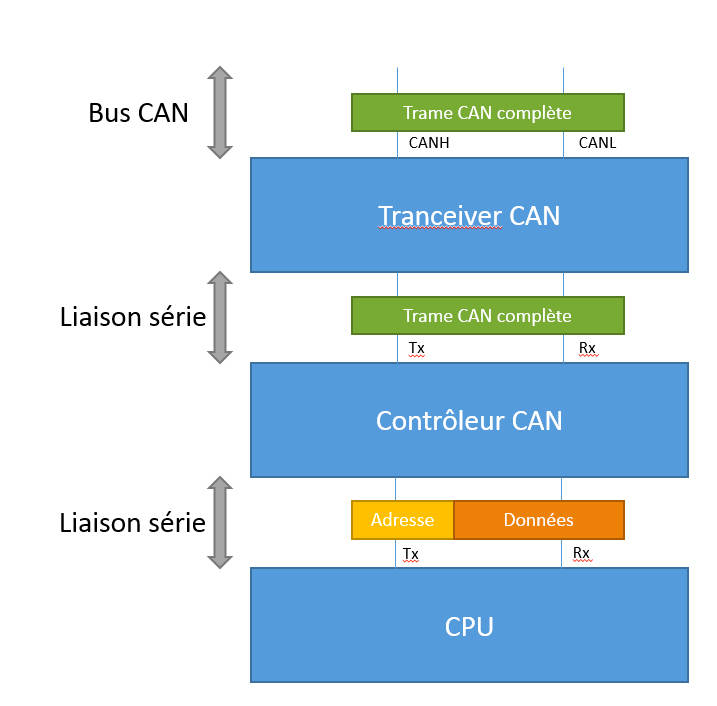
\includegraphics[width=0.7\textwidth]{schema.jpg}
\caption{Fonctionnement CPU <-> CAN}
\end{figure}

\subsection{Les trames ne transportent qu'un octet de données. Quelle est la durée approximative d'une trame ?}

Le débit de ce CAN est de $1Mbps$. Dans une trame CAN, on a $1+11+1+6+15+1+1+1+7+3+8*n_{octets}$ bits, soit ici 55 bits. La durée approximative d'une trame est donc de \SI{55}{\micro\second}.

\section{La trame CAN}

\subsection{Une fois les signaux affichés, à l'aide de la touche SAVE, récupérez le signal sur votre clé et imprimez-le. Décomposez alors la trame en champs principaux. Retrouvez la valeur de l'identifiant et des données.}

\begin{figure}[H]
\centering
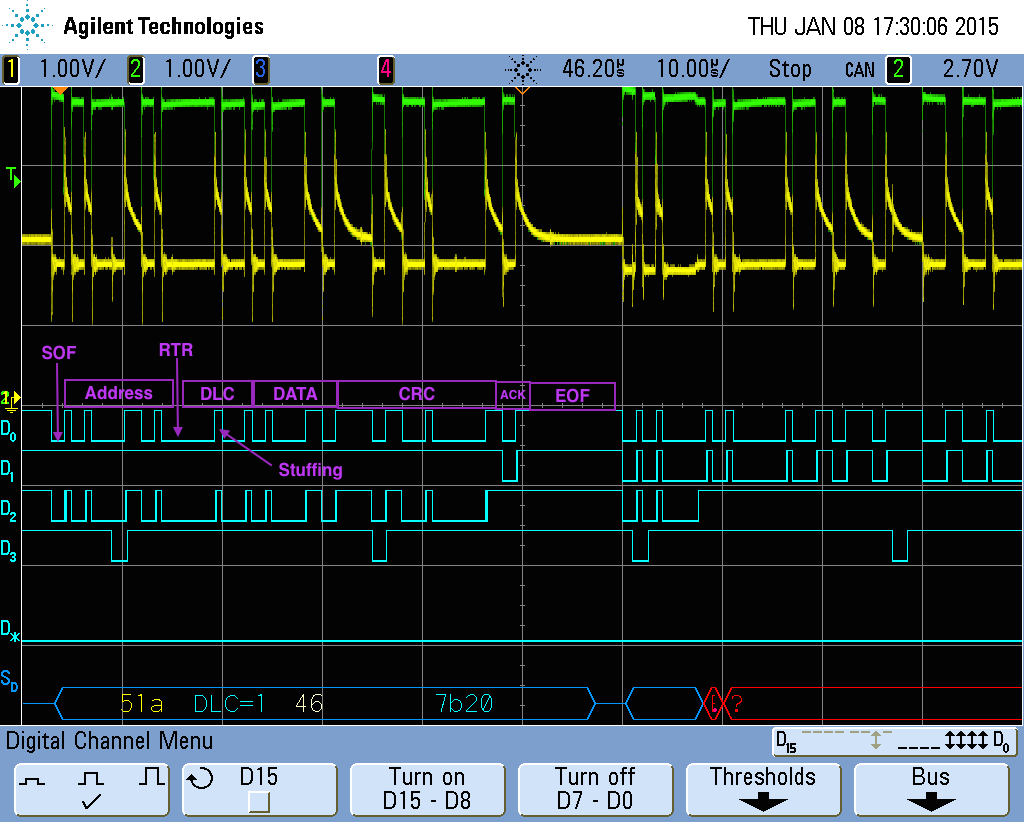
\includegraphics[width=0.9\textwidth]{releve_1.png}
\caption{Capture d'une trame CAN}
\end{figure}

La décomposition de la trame est annotée en violet sur la capture. On peut donc y lire que l'identifiant est $51A$ et que l'octet de données vaut $46$.

\subsection{Quelle est la trame de plus grande priorité ?}

La trame de plus grande priorité est la trame donc l'adresse est la plus faible. Ici, par ordre de priorité, on a donc la valeur du potentiomètre 0 (adresse $50A$), la valeur du potentiomètre 1 (adresse $51A$), puis la valeur du potentiomètre 2 (adresse $52A$).

\subsection{La trame donnant la valeur envoyée par le noeud 2 apparaît-elle ? Pourquoi ? Montrez sur votre relevé de signaux comment se fait l'arbitrage.}

La trame envoyée par le noeud 2 n'apparaît jamais, car elle est toujours écrasé par les trames $50A$ et $51A$, qui sont émises trop fréquemment pour que $52A$ ait le droit à la parole sur le bus.

\begin{figure}[H]
\centering
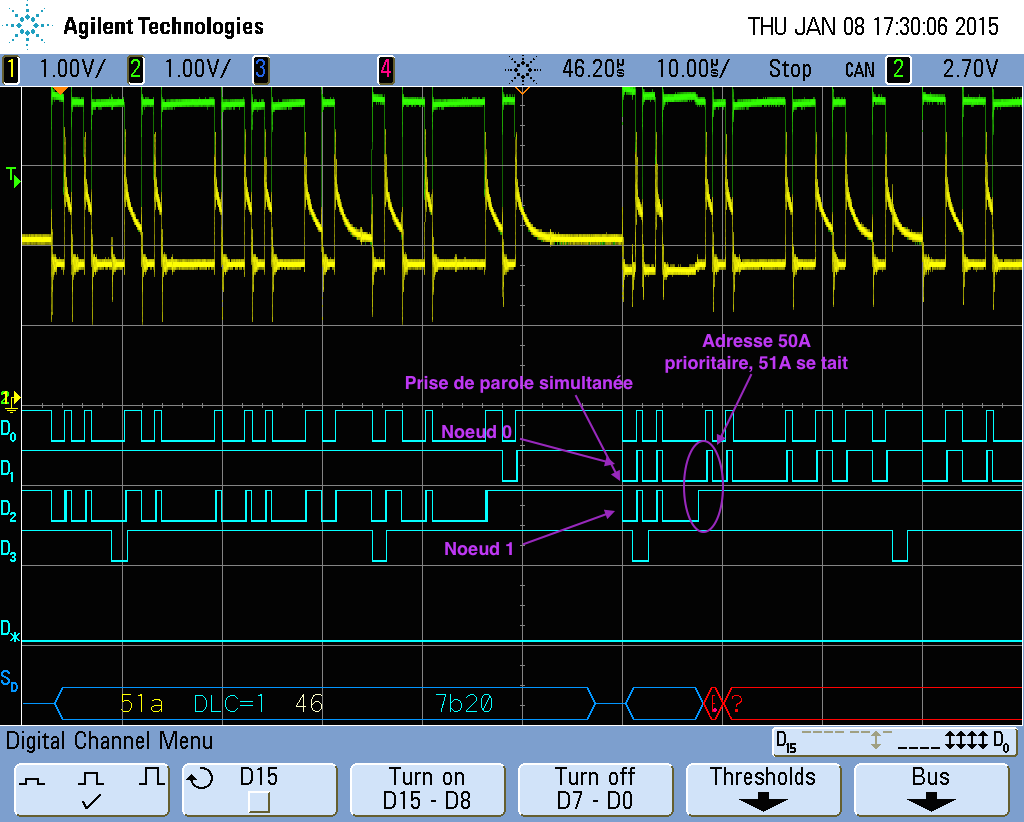
\includegraphics[width=0.9\textwidth]{releve_2.png}
\caption{Démonstration d'un arbitrage}
\end{figure}

\section{Tolérance sur les horloges}

\subsection{A partir de quelles valeurs voyez-vous apparaître des erreurs de réception ou transmission ?}

En dehors de la plage $[7800kHz, 8130kHz]$, les erreurs commencent à apparaitre.

\subsection{Le bus CAN est-il synchrone ou asynchrone ? Que pouvez-vous dire sur la tolérance des horloges du bus CAN ?}

Le bus CAN est asynchrone, le resynchronisation des horloges se faisant à partir du signal lui-même. La tolérance mesurée ici est de l'ordre de $2\%$, ce qui est relativement élevé. Le bus CAN est donc très tolérant sur les horloges.

\subsection{Cela correspond-il à la théorie ?}

Cette grande tolérance correspond parfaitement à la théorie. En effet, les horloges des noeuds CAN sont souvents des composants peu chers, tels que des quartz. D'autre part, dans le cas d'un CAN embarqué sur une automobile, les différences de température en un noeud placé sous le capot et un noeud placé à l'air libre induisent des décalages des horloges, auxquels le protocole doit pouvoir résister, afin de garantir un bon fonctionnement de l'automobile dans des conditions climatiques rudes.

\subsection{Expliquez l'intérêt des bits de stuffing}

Les bits de stuffing ont un intérêt double. D'une part, ils permettent de distinguer une longue série de 0 d'une trame d'erreur. D'autre part, ils permettent de ne pas laisser une trop longue série de bits identiques se succéder, et d'assurer ainsi une bonne synchronisation des horloges quel que soit le message à transmettre/recevoir.

\subsection{Quel est l'intérêt de l'oscilloscope (environ 6000 euros) par rapport à l'analyseur de bus CAN présent sur les maquettes (environ 50 euros) ?}

L'intérêt de l'oscilloscope est de pouvoir analyser n'importe quel signal passant sur le bus. Contrairement à l'analyseur, il est possible avec l'oscilloscope de détecter des trames d'erreurs, des problèmes liés aux transceivers, au bus, etc... L'oscilloscope affichera dans tous les cas la donnée brute, l'analyseur n'affichera la donnée que si elle est correcte.

\end{document}